\chapter{Evaluation und Validation}
\label{ch:Eval}

Um das System zu validieren und die Grenzen der Infrarotbildverarbeitung in diesem Gebiet zu ermitteln wurden einige Experimente durchgeführt. Diese Experimente zeigen was das System kann und wo die Grenzen des Systems und auch der Infrarottechnik liegen.\\
\\
Zur Auswertung der Experimente werden Bilder mit Markierungen verwendet. Diese sind wie folgt Farbcodiert.
\begin{itemize}
	\item Grün -> Korrekt gefundene Person (True Positive)
	\item Gelb -> Nicht gefundene Person (False Negative)
	\item Rot -> Nichtiger Treffer (False Positive)
\end{itemize}

\section{Vergleich mit Anforderungen}
\label{sec:VergleichAnforderungen}

Die Aufgabe war es ein System zu entwickeln welches in dem Sitzungszimmer auf den Bildern der Infrarotkameras die Anzahl und Position der Personen ermittelt. Dieser Punkt wurde erfüllt. Das System kann dynamisch Personen und deren Position ermitteln und diese ausgeben. Das System zeigte bei den Tests wie in Abbildung \ref{fig:ExperimentSummary} zu sehen eine Precision Score von 97\% das bedeutet, dass es fast gar keine False Positives gab. Die Accuracy liegt nur bei 85\%, dies weil in den Experimenten auch die Grenzen der Personenerkennung getestet werden wie in Kapitel \ref{sec:cloths} diskutiert wird.

\begin{figure}[H]
	\centering
	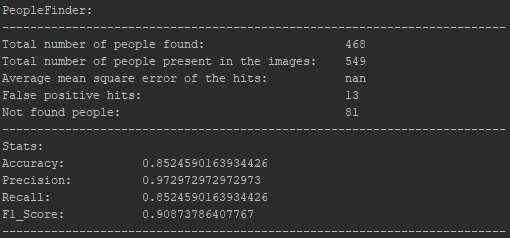
\includegraphics[width=.9\linewidth]{ExperimentSummary}
	\caption{Zusammenfassung aller ergebnisse der Experimente}
	\label{fig:ExperimentSummary}
\end{figure}



\section{Fremde Wärmequellen}
\label{sec:FremdeWärmequellen}

In diesem Versuch wurde der Einfluss von fremden Wärmequellen wie zum Beispiel Laptops, Natels, oder Kaffees, evaluiert. Dabei wurde der Effekt von Störquellen mit und ohne Personen im Raum analysiert.

\subsection{Resultate}
\label{subsec:FWresultate}

Der Threshold-Algorithmus kann wie erwartet nicht gut mit anderen Wärmequellen umgehen. Dies, weil der Threshold-Algorithmus nur durch Temperatur und Mindestgrösse eines Objekts entscheiden kann ob es sich um eine Person handelt. Deshalb hatte dieser bei einem Experiment mit einer Person und einem Laptop, nur eine Precision Score von 64\% erreicht (Siehe Abbildung \ref{fig:ThreshPersonLaptop}).

Das \gls{CNN} kann sehr gut mit anderen Wärmequellen umgehen, solange diese in ähnlicher Form antrainiert wurden. Dabei ist es von Vorteil, dass in einem Sitzungszimmer nicht viele unterschiedliche Wärmequellen vorkommen.

\vspace{.5em}
\begin{figure}[H]
	\begin{subfigure}{.45\linewidth}
		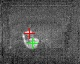
\includegraphics[keepaspectratio,height=4cm]{ThreshPersonLaptop}
		\caption{Ergebnis der Threshold-Methode des Experiments mit Laptop und Person}
		\label{fig:ThreshPersonLaptop}
	\end{subfigure}\hfill%
	\begin{subfigure}{.45\linewidth}
		\centering
		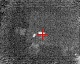
\includegraphics[keepaspectratio,height=4cm]{ThresholdLaptop}
		\caption{Threshold-Methode Ergebnis des Experiments mit nur einem Laptop}
		\label{fig:thresholdDistanice10}
	\end{subfigure}
	\begin{subfigure}{\linewidth}
		\centering
		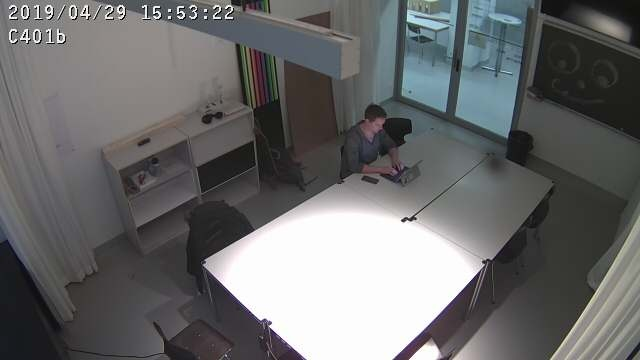
\includegraphics[keepaspectratio,height=3cm]{GroundHeatSources}
		\caption{Ground-Truth des Experiments mit Laptop und Person}
		\label{fig:groundDiistance10}
	\end{subfigure}
	\caption{Experimente mit fremden Wärmequellen}
	\label{fig:HeatSources}
\end{figure}
\vspace{.5em}



\section{Distanz}
\label{sec:distanz}

Die Distanz zwischen zwei Personen ist ein wichtiger Faktor, der sich gleichermassen auf die Threshold-Methode auswirkt, wie auch auf das \gls{CNN}. Da bei dem \gls{CNN} mit einer Sliding-Window Methode und clustern der Treffer gearbeitet wird, kann das System bei Personen, welche zu wenig Abstand zueinander haben, nicht mehr zwischen den Treffern unterscheiden. Bei der Threshold-Methode wird die Silhouette der Personen leicht vergrössert, wodurch mehrere Personen bei geringem Abstand als einzelner Treffer gewertet werden.

\subsection{Resultate}

Die Algorithmen können Personen bereits ab einem Abstand von 10cm auseinanderhalten, sofern die Personen so ausgerichtet sind, dass die optische Verzerrung keinen Einfluss auf den Zwischenraum hat. Wie in den Abbildungen und auf der linken Seite zu sehen, wenn die Personen auf die Kamera ausgerichtet sind, können sie unterschieden werden. Sind die Personen wie auf der rechten Seite von der Kamera aus gesehen hintereinander kann bei so kleinem Abstand nicht ermittelt werden, ob es sich um eine oder zwei Personen handelt.\\
\\
Befinden sich die Personen in der schlechtest möglichen Position benötigen die Algorithmen einen Mindestabstand von 30cm um die Personen fehlerfrei unterscheiden zu können. Siehe Abbildungen \ref{fig:cnnDistance30} und \ref{fig:thresholdDistance30}

\begin{figure}[H]
	\begin{subfigure}{.45\linewidth}
		\centering
		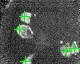
\includegraphics[keepaspectratio,height=4cm]{CNNDistance10}
		\caption{\gls{CNN} Ergebnis des Distanztest mit 10cm Abstand}
		\label{fig:cnnDistance10}
	\end{subfigure}\hfill%
	\begin{subfigure}{.45\linewidth}
		\centering
		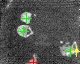
\includegraphics[keepaspectratio,height=4cm]{ThresholdDistance10}
		\caption{Threshold Ergebnis des Distanztest mit 10cm Abstand}
		\label{fig:thresholdDistance10}
	\end{subfigure}
	\begin{subfigure}{\linewidth}
		\centering
		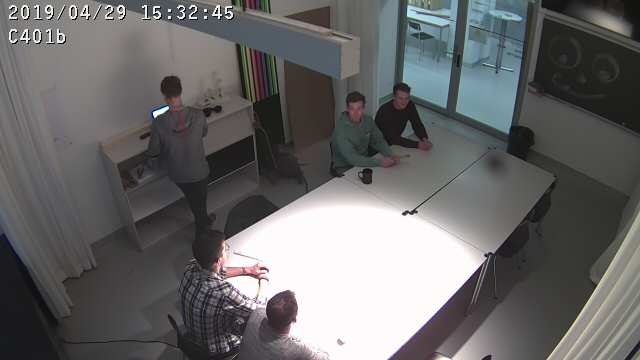
\includegraphics[keepaspectratio,height=3cm]{GroundDistance10}
		\caption{Ground-Truth Distanzexperiment mit 10cm Abstand}
		\label{fig:groundDistance10}
	\end{subfigure}
	\caption{Distanz Experiment 10cm}
	\label{fig:Distance10}
\end{figure}



\begin{figure}[H]
	\begin{subfigure}{.45\linewidth}
		\centering
		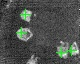
\includegraphics[keepaspectratio,height=4cm]{CNNDistance30}
		\caption{CNN Ergebnis des Distanztest mit 30cm Abstand}
		\label{fig:cnnDistance30}
	\end{subfigure}\hfill%
	\begin{subfigure}{.45\linewidth}
		\centering
		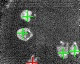
\includegraphics[keepaspectratio,height=4cm]{ThresholdDistance30}
		\caption{Threshold Ergebnis des Distanztest mit 30cm Abstand}
		\label{fig:thresholdDistance30}
	\end{subfigure}
	\begin{subfigure}{\linewidth}
		\centering
		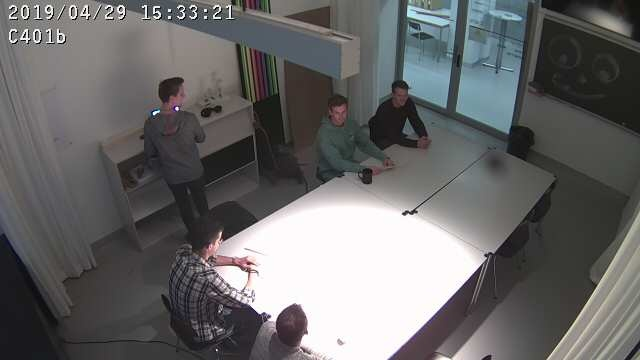
\includegraphics[keepaspectratio,height=3cm]{GroundDistance30}
		\caption{Ground-Truth}
		\label{fig:groundDistance30}
	\end{subfigure}
	\caption{Distanz Experiment 30cm}
	\label{fig:Distance30}
\end{figure}

\section{Kamerahöhe}
\label{sec:cameraHeight}
Eine Spezialität des Sitzungszimmers das zur Verfügung gestellt wurde ist, dass die Höhe der Decke verändert werden kann. Da die Infrarotkameras an der Decke montiert sind kann die Möglichkeit, dass die Decke verstellt wird, nicht ausser acht gelassen werden. Deshalb wurde auch dazu ein Experiment durchgeführt. Dabei wurden Minimal- und Maximalhöhe analysiert.

\subsection{Resultate}
Beide Algorithmen können Sehr gut mit dem verstellen der Decke umgehen. Das einzige Problem ist, dass umso tiefer die Decke eingestellt ist umso kleiner ist die Fläche im Raum die von den Infrarotkameras aufgenommen wird. Anderweitig hat die Deckenhöhe keinen Einfluss auf die Algorithmen.\\
Wenn die Position der Personen auf den realen Raum abgebildet werden soll, muss die Deckenhöhe zusätzlich berechnet oder gemessen werden.


\section{Kleider}
\label{sec:cloths}

Infrarotbilder zeigen die Wärmeabstrahlung der verschiedenen Objekte im Bild. Wird eine Wärmequelle isoliert verschwindet sie auf dem Infrarotbild. Genau das Passiert wenn stark isolierende Kleider getragen werden. Da in dieser Arbeit die Vogelperspektive analysiert wird sind vor allem Kopfbedeckungen und Schals ein grosser Einfluss.

\subsection{Resultate}
Kleider beeinflussen die Performance der Algorithmen massiv. Trägt eine Person eine Mütze wird sie vom \gls{CNN} noch zu 80\% erkannt. Bei der Threshold-Methode kann es dazu führen, dass eine Person zwei Treffer erzeugt(Siehe Abbildung \ref{fig:thresholdClothHat}).\\
\\
Wenn ein Schal getragen wird sinkt die Accuracy auf ca. 60\% bei Beiden Algorithmen. Betrachtet man Abbildung \ref{fig:scarfIR} sieht man deutlich, wie der Schal einen Teil der Wärme der Person verdeckt.\\
\\
Das Tragen einer Jacke macht es für die Algorithmen beinahe unmöglich die Personen zu erkenne. Die Person wird nur noch in wenigen Fällen erkannt. Das \gls{CNN} könnte wahrscheinlich mit den entsprechenden

\begin{figure}[H]
	\begin{subfigure}{.45\linewidth}
		\centering
		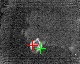
\includegraphics[keepaspectratio, height=4cm]{thresholdClothHat}
		\caption{Resultat der Threshold-Methode des Experiments mit Kopfbedeckung}
		\label{fig:thresholdClothHat}
	\end{subfigure}
	\begin{subfigure}{.45\linewidth}
		\centering
		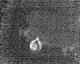
\includegraphics[keepaspectratio, height=4cm]{scarfIR}
		\caption{Infrarotbild einer Person die einen Schal trägt}
		\label{fig:scarfIR}
	\end{subfigure}
	
\end{figure}


Die Tests zeigen schon bei der manuellen, visuellen Analyse der Abbildung \ref{fig:rawClothAll}, dass wenn Jacke Mütze und Schal zusammen getragen werden, man die Person nicht mehr erkennen kann.

\begin{figure}[H]
	\begin{subfigure}{.45\linewidth}
		\centering
		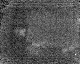
\includegraphics[keepaspectratio, height=4cm]{rawClothAll}
		\caption{Infrarotbild des Experiments mit Jacke Mütze und Schal}
		\label{fig:rawClothAll}
	\end{subfigure}
	\begin{subfigure}{.45\linewidth}
		\centering
		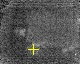
\includegraphics[keepaspectratio, height=4cm]{clothAll}
		\caption{Position der Person}
		\label{fig:AlgorithmsClothAll}
	\end{subfigure}
	\begin{subfigure}{\linewidth}
		\centering
		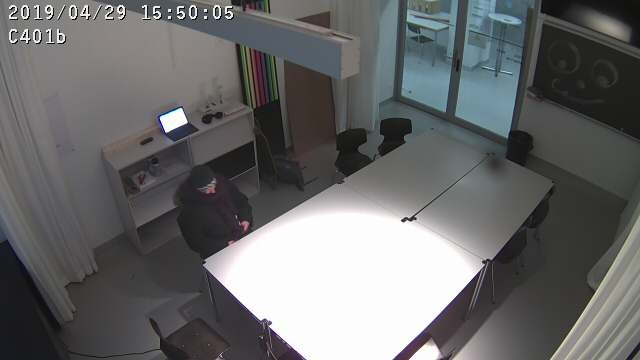
\includegraphics[keepaspectratio, width=.5\linewidth]{GroundClothAll}
		\caption{Ground-Truth des Experiments mit allen Kleidern}
		\label{fig:groundTruthClothAll}
	\end{subfigure}
	\caption{Experiment mit Jacke Mütze und Schal}
	\label{fig:AllCloth}
\end{figure}

